\subsection{3D Modell\hfill\textnormal{\emph{Berger}}}

Der grundsätzliche Aufbau des Roboters hat sich nach dem kombinierten Prototypen nicht stark verändert.
Die Aufgabe des finalen Modells war es also 
genauer zu definieren aus welchen Bauteilen der Roboter besteht
und zu beweisen das alle angedachten Funktionen im Gerät unterzubringen sind.

Wie in Abbildung \ref{fig:model_open_front} zu sehen, 
besteht der finale Roboter aus einer großen Grundplatte, 
die durch eine Rückwand und einen Deckel abgedeckt wird.
Dies vereinfacht die Wartung der inneren Komponenten
und erlaubt das komplette ausbauen der beiden Container.(NFR9)

\begin{figure}[H]
  \centering{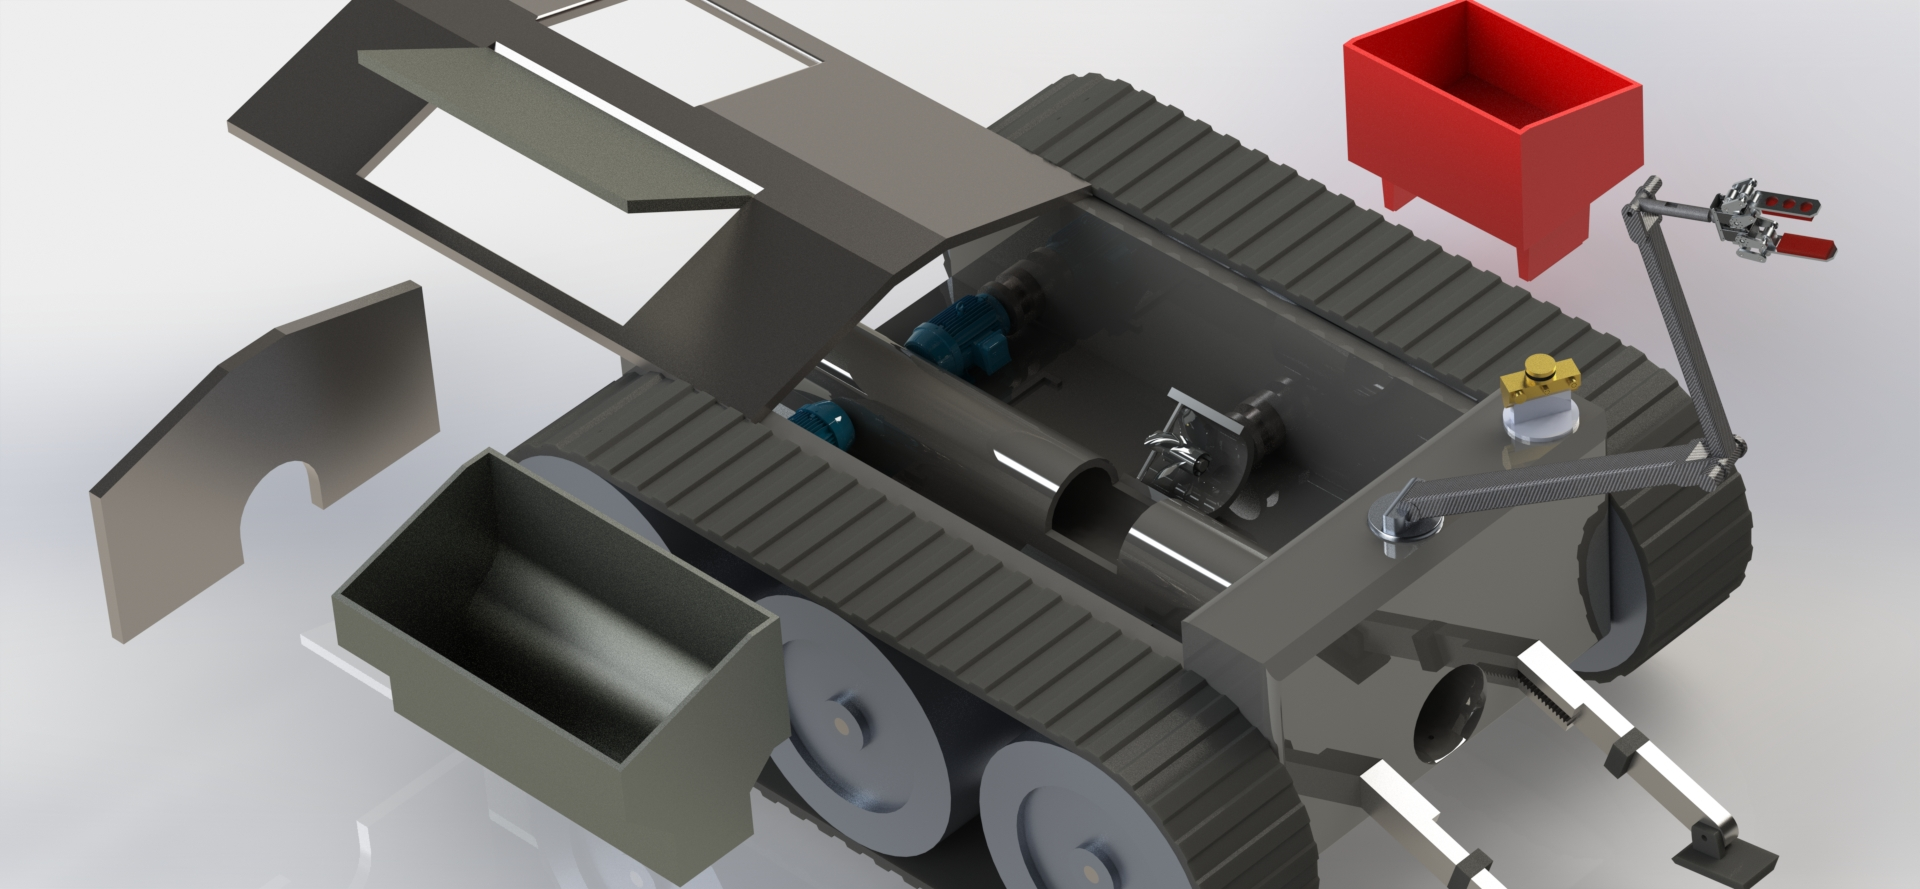
\includegraphics[width=1.0\linewidth]{Abbildungen/3D_model/final_open_front_2.JPG}}
  \caption{Modell final TEST}
  \label{fig:model_open_front}
\end{figure}

Wie in Abbildung \ref{fig:model_open_front} zu erkennen
wurde der Greifarm des Roboters im Vergleich zum Prototypen deutlich verstärkt.
Dies verbessert die Fähigkeit des Arms besonders schwere Objekte zu bergen.(FR3)
Als Material für den Greifarm wurde vorerst Carbonfasern gewählt,
gut zu sehen in Abbildung \ref{fig:model_closeup}.
Dies wurde gemacht um die Hebelwirkung des Arms zu verringern,
wenn dieser sich auf weite Distanzen ausstreckt.
Ob die Konstruktion aus dem Material stark genug ist 
um auch schwere Objekte zu bergen,
muss noch getestet werden und könnte die Wahl des Materials noch verändern.

Die Ketten wurden um relativ sanfte Zähne erweitert 
um die Griff-Fähigkeit auf losem Untergrund zu verbessern.(FR1, NFR1)
Sie werden angetrieben durch jeweils einen Elektromotor,
der am hinteren Rad angebracht ist,
besonders gut zu sehen in Abbildung \ref{fig:model_open_back}.

In der Mitte der Grundplatte befindet sich eine Aussparung in der Wasser-Röhre.
Dort wird der Propeller an einer Klappe befestigt,
die wie in Abbildung \ref{fig:model_open_front} gezeigt
aufgeklappt werden kann, 
zur Installation oder Wartung.(NFR9)
Am Ende der Röhre befindet sich das Ruder, 
wie in Abbildung \ref{fig:model_open_back} zu sehen.(FR2, NFR2)

\begin{figure}[H]
  \centering{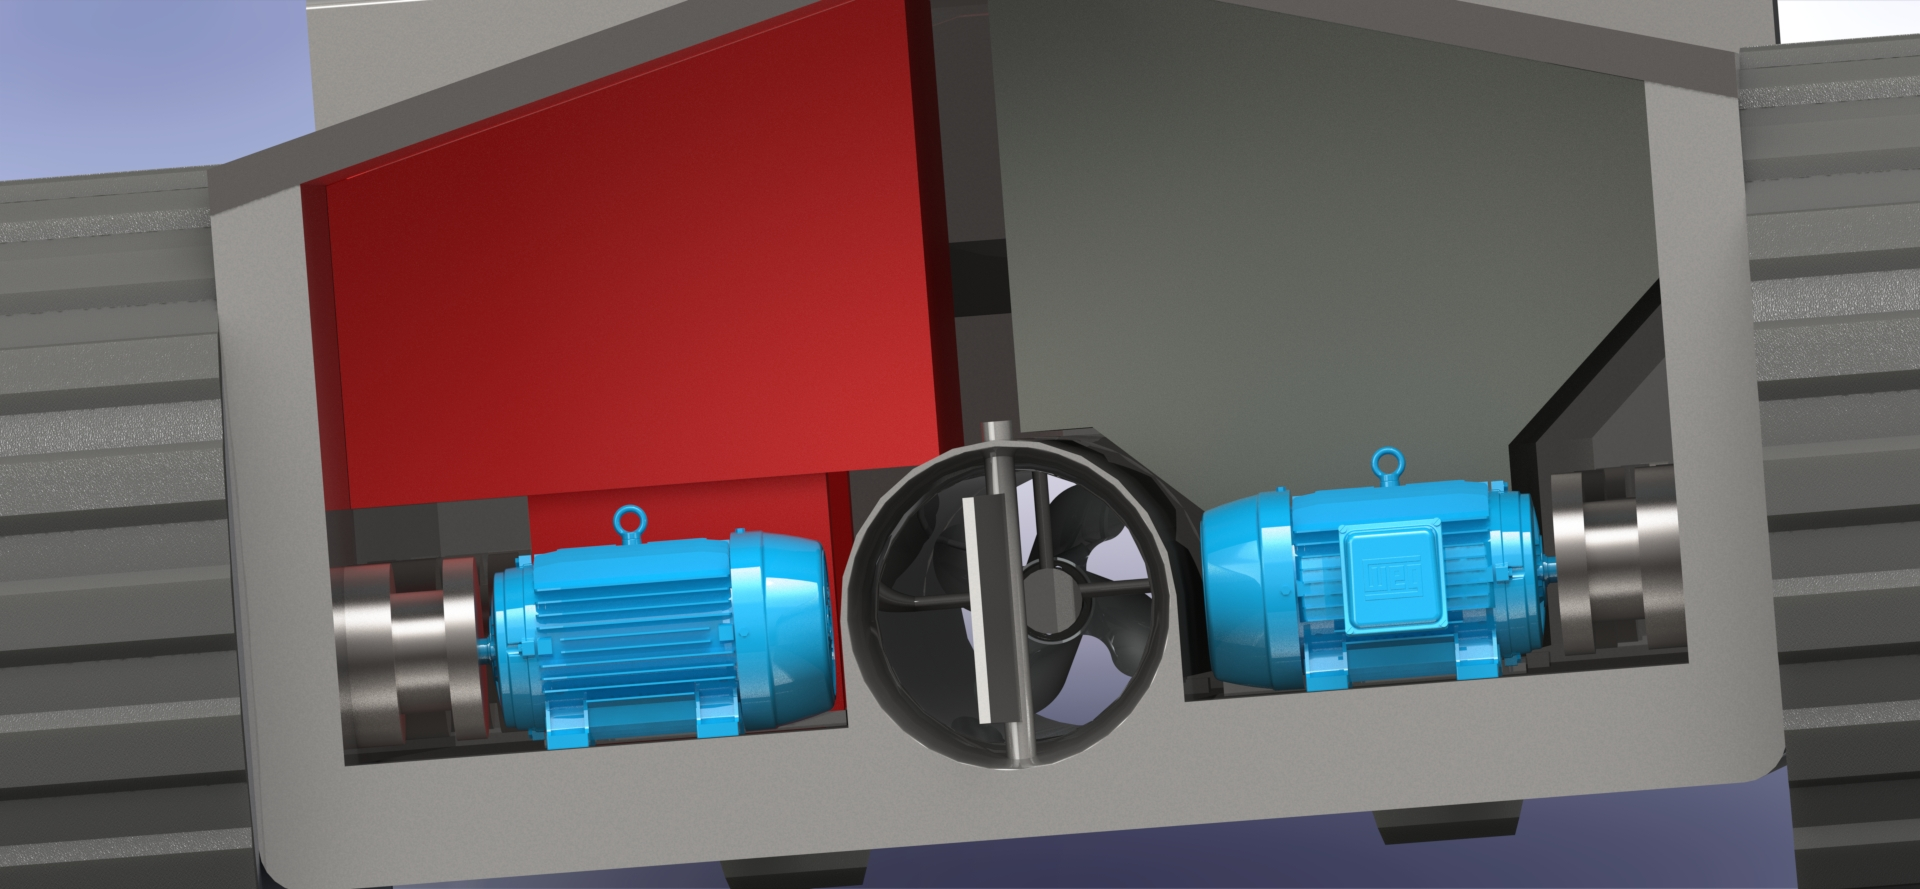
\includegraphics[width=1.0\linewidth]{Abbildungen/3D_model/final_open_back.JPG}}
  \caption{Modell back}
  \label{fig:model_open_back}
\end{figure}

Die beiden Container werden mit einfach von oben in den Roboter eingesetzt.
Sie werden festgehalten von dem Deckel und den Seitenwänden,
sowie von kleinen Erhebungen in der Grundplatte,
die die Füße der Container umschließen.
Die Klappe die den rechten Container verschließt ist in dem Deckel integriert.(FR4)

Die Stützen an der Vorderseite blieben im Ansatz gleich,
wurden aber durch eine Gummi-Dichtung in der Mitte des Beins erweitert,
zu sehen unten rechts in Abbildung \ref{fig:model_open_front}.
Sobald der Roboter Wasser erkennt, 
können die Stützen komplett eingefahren werden,
wodurch die Dichtungen das sonst leicht durchlässige Loch im Chassis abdichten.

\begin{figure}[H]
  \centering{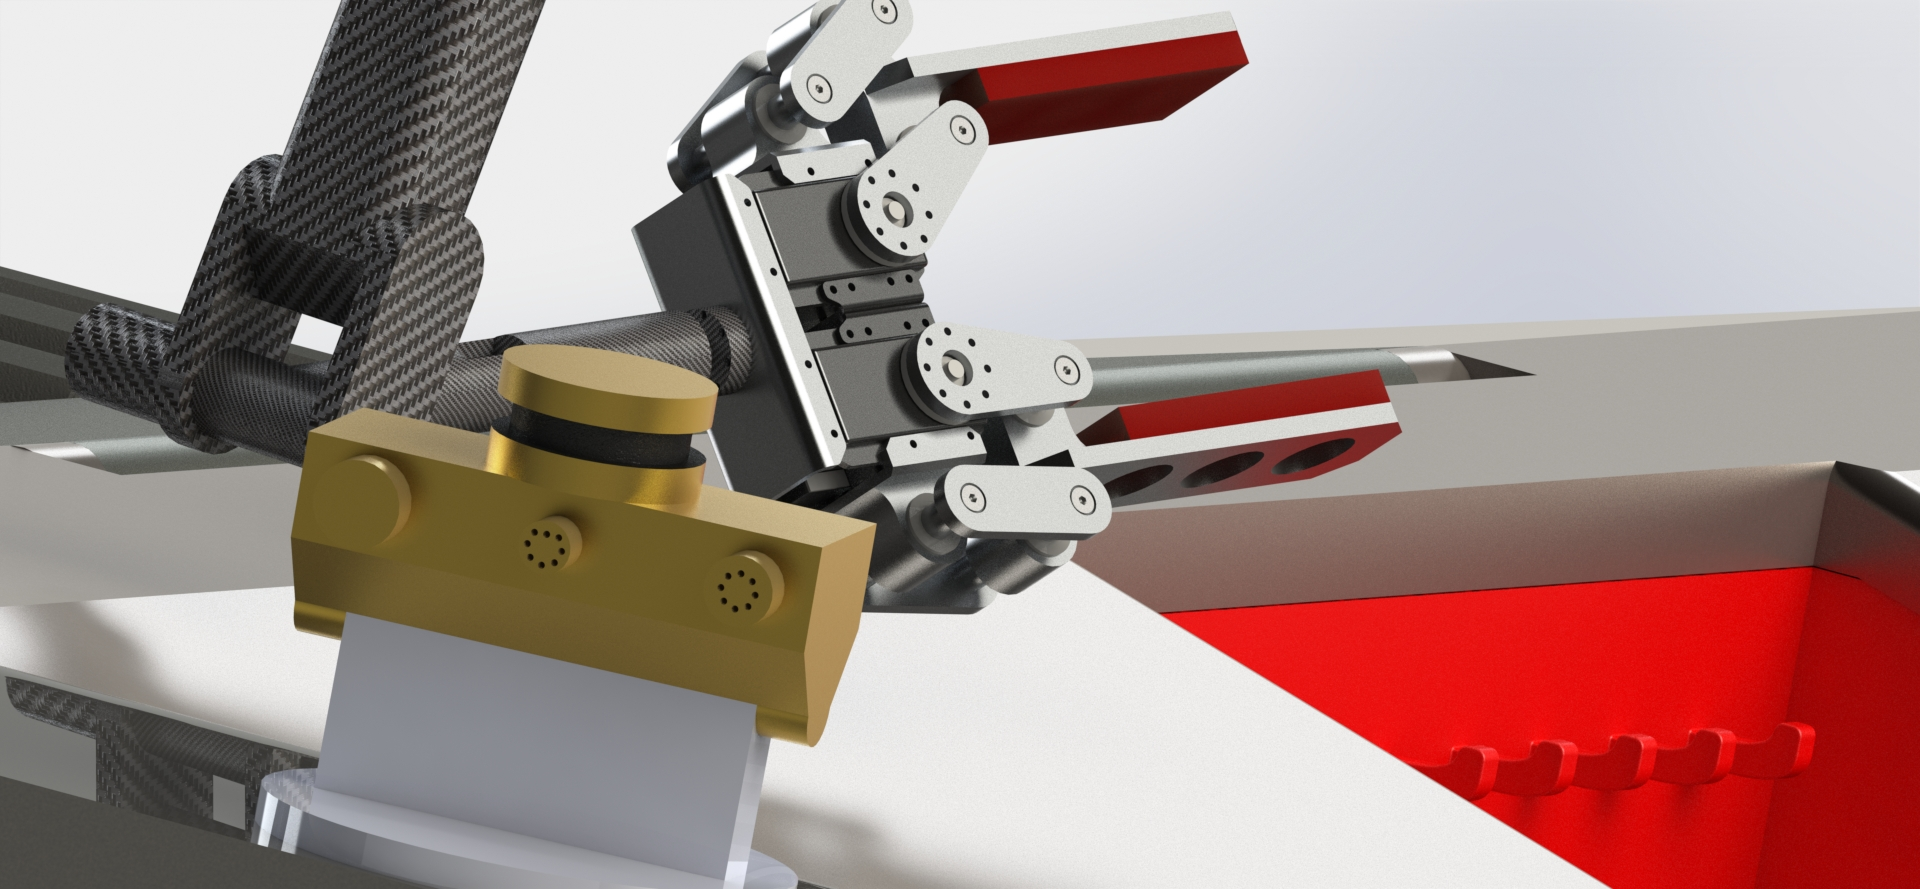
\includegraphics[width=1.0\linewidth]{Abbildungen/3D_model/Final_utility_closeup.JPG}}
  \caption{Werkzeuge des Roboters}
  \label{fig:model_closeup}
\end{figure}

Abbildung \ref{fig:model_closeup} zeigt deutlich den Aufbau von dem Sensor-Array und dem Greifer.
Der Lautsprecher und die Kamera, Mikrofon und LIDAR Sensoren 
befinden sich auf einer kipp- und drehbaren Halterung.
Dies ermöglicht die komplette Aufnahme der Umgebung.(NFR8)

Der Greifer ist angetrieben von 2 Motoren und setzt deren Drehbewegung 
in eine parallele Bewegung der Greifer-Platten in rot um.
Dies ermöglicht sanftes und rutschfestes Greifen von viele unterschiedlichen Formen.(NFR3.1)

Rechts im Hintergrund von Abbildung \ref{fig:model_closeup} befindet sich der offene Container.
Zu erkennen sind die vier Haken, 
an denen eventuelles Erste-Hilfe-Material oder ähnliches auf gehangen werden kann,
um den Container aufgeräumt zu halten.(NFR5)

